\documentclass[
	10pt,								% globale Schriftgröße
	parskip=half-,						% setzt Absatzabstand hoch
	paper=a4,							% Format
	english,ngerman,					% lädt Sprachpakete
	]{scrartcl}							% Dokumentenklasse

% //////////////////// Pakete laden ////////////////////
\usepackage[fleqn]{amsmath}
\usepackage[fleqn]{mathtools}
\usepackage{amssymb}			% mathematische symbole, für \ceckmarks
\usepackage{amsthm}				% für proof
\usepackage{mathrsfs}			% für \mathscr
\usepackage{latexsym}
\usepackage{marvosym}				% für Lightning

\usepackage{fontspec} 			% funktioniert nur mit den neueren Compilern z.B. XeLaTeX
\usepackage{microtype}			% für bessere Worttrennung
\usepackage[ngerman]{babel} 	% Spracheinstellung
\usepackage{lmodern}			% verändert verwendete Schriftart, damit sie weniger pixelig ist

\usepackage{verbatim}
\usepackage{listings}			% Für Quellcode

\usepackage{graphicx}
\usepackage{tabularx}			% für Tabellen mit gleicher Spaltenbreite und automatischen Umbrüchen
\usepackage{fullpage}
\usepackage{multirow}			% für multirow in tabulars
\usepackage{rotate}
\usepackage[cmyk,table]{xcolor} % um Farben zu benutzen, kann mehr als das Paket color
\usepackage[					% Verlinkungen
	colorlinks,					% farbige Schrift, statt farbiger Rahmen
	linktocpage,				% verlinkt im Abb.Verzeichnis Seitenzahl statt Bildunterschrift
	linkcolor=blue				% setzt Farbe der Links auf blau
	]{hyperref}					% nur für digitale Anwendungen, url = "http://www.example.com"
\usepackage{url}				% für Webadressen wie e-mail usw.: "\url{http://www.example.com}"

\usepackage{enumerate}			% für versch. Aufzählungezeichen wie z.B. a)
\usepackage{xspace}				% folgt ein Leerzeichen nach einem \Befehl, wird es nicht verschluckt.
\usepackage{cancel}				% für das Durchstreichen u.a. in Matheformeln mit \cancel
\usepackage{float}              % zum Forcieren der Position von figure-Umgebungen

% zum Zeichnen (u.a. von Graphen)
\usepackage{fp}
\usepackage{tikz}
\usetikzlibrary{tikzmark}			% für \tikzmark{toRemember}
\usetikzlibrary{positioning}	% verbesserte Positionierung der Knoten
\usetikzlibrary{automata}		% für Automaten (GTI)
\usetikzlibrary{arrows}
\usetikzlibrary{shapes}
\usetikzlibrary{decorations.pathmorphing}
\usetikzlibrary{decorations.pathreplacing}
\usetikzlibrary{decorations.shapes}
\usetikzlibrary{decorations.text}

% //////////////////// Syntaxhighlighting ////////////////////
\lstloadlanguages{Python, Haskell, [LaTeX]TeX, Java}
\lstset{
   basicstyle=\footnotesize\ttfamily,	% \scriptsize the size of the fonts that are used for the code
   backgroundcolor = \color{bgcolour},	% legt Farbe der Box fest
   breakatwhitespace=false,	% sets if automatic breaks should only happen at whitespace
   breaklines=true,			% sets automatic line breaking
   captionpos=t,				% sets the caption-position to bottom, t for top
   commentstyle=\color{codeblue}\ttfamily,% comment style
   frame=single,				% adds a frame around the code
   keepspaces=true,			% keeps spaces in text, useful for keeping indentation
							% of code (possibly needs columns=flexible)
   keywordstyle=\bfseries\ttfamily\color{codepurple},% keyword style
   numbers=left,				% where to put the line-numbers;
   							% possible values are (none, left, right)
   numberstyle=\tiny\color{codegreen},	% the style that is used for the line-numbers
   numbersep=5pt,			% how far the line-numbers are from the code
   stepnumber=1,				% nummeriert nur jede i-te Zeile
   showspaces=false,			% show spaces everywhere adding particular underscores;
							% it overrides 'showstringspaces'
   showstringspaces=false,	% underline spaces within strings only
   showtabs=false,			% show tabs within strings adding particular underscores
   flexiblecolumns=false,
   tabsize=1,				% the step between two line-numbers. If 1: each line will be numbered
   stringstyle=\color{orange}\ttfamily,	% string literal style
   numberblanklines=false,				% leere Zeilen werden nicht mitnummeriert
   xleftmargin=1.2em,					% Abstand zum linken Layoutrand
   xrightmargin=0.4em,					% Abstand zum rechten Layoutrand
   aboveskip=2ex, 
}

\lstdefinestyle{py}{
   language=Python,
}
\lstdefinestyle{hs}{
   language=Haskell,
}
\lstdefinestyle{tex}{
	language=[LaTeX]TeX,
	escapeinside={\%*}{*)},     % if you want to add LaTeX within your code
	texcsstyle=*\bfseries\color{blue},% hervorhebung der tex-Schlüsselwörter
	morekeywords={*,$,\{,\},\[,\],lstinputlisting,includegraphics,
	rowcolor,columncolor,listoffigures,lstlistoflistings,
	subsection,subsubsection,textcolor,tableofcontents,colorbox,
	fcolorbox,definecolor,cellcolor,url,linktocpage,subtitle,
	subject,maketitle,usetikzlibrary,node,path,addbibresource,
	printbibliography},% if you want to add more keywords to the set
     numbers=none,
     numbersep=0pt,
     xleftmargin=0.4em,
}

\lstdefinestyle{java}{
	language=Java,
	extendedchars=true,		% lets you use non-ASCII characters;
   						% for 8-bits encodings only, does not work with UTF-8
}

\lstdefinelanguage[x64]{Assembler}     % add a "x64" dialect of Assembler
   [x86masm]{Assembler} % based on the "x86masm" dialect
   % with these extra keywords:
   {morekeywords={CDQE,CQO,CMPSQ,CMPXCHG16B,JRCXZ,LODSQ,MOVSXD, %
                  POPFQ,PUSHFQ,SCASQ,STOSQ,IRETQ,RDTSCP,SWAPGS, %
                  rax,rdx,rcx,rbx,rsi,rdi,rsp,rbp, %
                  r8,r8d,r8w,r8b,r9,r9d,r9w,r9b}
}					% for 8-bits encodings only, does not work with UTF-8

\lstdefinestyle{c}{
	language=c,
	extendedchars=true,		% for 8-bits encodings only, does not work with UTF-8
}

% //////////////////// eigene Kommandos ////////////////////
\newcommand\FU{Freie Universität Berlin\xspace}% benötigt package xspace
\newcommand\gdw{g.\,d.\,w.\xspace}
\newcommand\oBdA{o.\,B.\,d.\,A.\xspace}
\newcommand{\Eu}{\texteuro}
\newcommand\N{\mathbb{N}\xspace}
\newcommand\Q{\mathbb{Q}\xspace}
\newcommand\R{\mathbb{R}\xspace}
\newcommand\Z{\mathbb{Z}\xspace}
\newcommand\ohneNull{\ensuremath{\backslash\lbrace 0\rbrace}}% \{0}
\let\dhALT\dh	% Schreibt Befehl \dh in \dhALT um
\renewcommand\dh{d.\,h.\xspace}	%renew überschreibt command \dh
\newcommand\Bolt{\;\text{\LARGE\raisebox{-0.3em}{\Lightning}\normalsize}\xspace}% Blitz
\newcommand\zz{\ensuremath{\raisebox{+0.25ex}{Z}% zu zeigen
			\kern-0.4em\raisebox{-0.25ex}{Z}%
			\;\xspace}}
\newcommand{\from}{\ensuremath{\colon}}
\newcommand{\floor}[1]{\lfloor{#1}\rfloor}
\newcommand{\ceil}[1]{\lceil{#1}\rceil}
 \renewcommand{\L}{\ensuremath{\mathcal{L}}\xspace}
 \renewcommand{\P}{\ensuremath{\mathcal{P}}\xspace}
 \newcommand{\NL}{\ensuremath{\mathcal{N}\kern-0.2em\mathcal{L}}\xspace}
 \newcommand{\NP}{\ensuremath{\mathcal{NP}}\xspace}

% //////////////////// Mathefunktionen ////////////////////
\DeclareMathOperator{\Landau}{\mathcal{O}}
\DeclareMathOperator{\True}{True}
\DeclareMathOperator{\False}{False}

% //////////////////// eigene Theoreme ////////////////////
\newtheorem{theorem}{Satz}
\newtheorem{corollary}[theorem]{Folgerung}
\newtheorem{lemma}[theorem]{Lemma}
\newtheorem{observation}[theorem]{Beobachtung}
\newtheorem{definition}[theorem]{Definition}
\newtheorem{Literatur}[theorem]{Literatur}
% konfiguriert proof
\makeatletter
\newenvironment{Proof}[1][\proofname]{\par
  \pushQED{\qed}%
  \normalfont \topsep6\p@\@plus6\p@\relax
  \trivlist
  \item[\hskip\labelsep
%         \itshape
        \bfseries
    #1\@addpunct{.}]\ignorespaces
}{%
  \popQED\endtrivlist\@endpefalse
}
\makeatother

% //////////////////// eigene Farben ////////////////////
\let\definecolor=\xdefinecolor
\definecolor{FUgreen}{RGB}{153,204,0}
\definecolor{FUblue}{RGB}{0,51,102}

\definecolor{middlegray}{rgb}{0.5,0.5,0.5}
\definecolor{lightgray}{rgb}{0.8,0.8,0.8}
\definecolor{orange}{rgb}{0.8,0.3,0.3}
\definecolor{azur}{rgb}{0,0.7,1}
\definecolor{yac}{rgb}{0.6,0.6,0.1}
\definecolor{Pink}{rgb}{1,0,0.6}

\definecolor{bgcolour}{rgb}{0.97,0.97,0.97}
\definecolor{codegreen}{rgb}{0,0.6,0}
\definecolor{codegray}{rgb}{0.35,0.35,0.35}
\definecolor{codepurple}{rgb}{0.58,0,0.82}
\definecolor{codeblue}{rgb}{0.4,0.5,1}

% //////////////////// eigene Settings ////////////////////

\textheight = 230mm		% Höhe des Satzspiegels / Layouts
\footskip = 10ex			% Abstand zw. Fußzeile und Grundlinie letzter Textzeile
\parindent 0pt			% verhindert Einrückung der 1. Zeile eines Absatzes
\setkomafont{sectioning}{\rmfamily\bfseries}% setzt Ü-Schriften in Serifen, {disposition}											% bindet Header ein (WICHTIG)
\usepackage{graphicx}
\usepackage{amsmath}
\usepackage{amssymb}
\usepackage{fancyvrb}

\newcommand{\dozent}{Prof. R. Rojas}					% <-- Names des Dozenten eintragen
\newcommand{\projectNo}{4}
\newcommand{\veranstaltung}{Mustererkennung}
\newcommand{\semester}{WS17/18}
\newcommand{\studenten}{Boyan Hristov, Nedeltscho Petrov}
% /////////////////////// BEGIN DOKUMENT /////////////////////////


\begin{document}
% /////////////////////// BEGIN TITLEPAGE /////////////////////////
\begin{titlepage}
	\subject{\dozent}
	\title{\veranstaltung, \semester}
	\subtitle{\Large Übungsblatt \projectNo\\ \large\vspace{1ex} }
	\author{\studenten}
	\date{\normalsize \today}
\end{titlepage}

\maketitle								% Erstellt das Titelblatt
\vspace*{-9cm}							% rückt Logo an den oberen Seitenrand
\makebox[\dimexpr\textwidth+1cm][r]{	%rechtsbündig und geht rechts 1cm über Layout hinaus
	
\includegraphics[width=0.4\textwidth]{src/fu_logo} % fügt FU-Logo ein
}
% /////////////////////// END TITLEPAGE /////////////////////////

\vspace{7cm}							% Abstand
\rule{\linewidth}{0.8pt}				% horizontale Linie										% erstellt die Titelseite


Link zum Git Repository: \url{https://github.com/BoyanH/FU-MachineLearning-17-18/tree/master/Solutions/Homework\projectNo}

\section*{Fischer Klassifikation}


\section*{Score (Output des Programs) bzw. Analyse}
Das ist die Ausgabe des Programs und damit auch das Score
\begin{lstlisting}
Best score for seed=879: 0.930510314875
Worst score for seed530: 0.880564603692
Score: 0.9305103148751357
Score with linear regression: 0.9055374592833876
\end{lstlisting}

Wie wir hier sehen, ist das Score auch sehr davon abhängig, wie man die Daten in Test und Train Sets
splitet. Es ist deswegen so, weil einige Emails sehr untypische spam Emails bzw nicht spam Emails sind.
Deswegen ist unser Score zwischen 88% und 93%.

Bei linearen Regression haben wir etwas schlechteres Ergebniss mit dem Datensatz bekommen (lineare Regression von
scikit-learn wurde benutzt). Das ist deswegen so, wie in der Vorlesung erklärt, weil die Kovarianzmatritzen in dem
Fall für Fischer Klassifizierung besser geeignet sind. Anders gesagt, die Streuung der Daten von je Klasse liegen
teilweise othogonal zu einander.

Aus performance-sichten haben wir nicht erkennbar bessere Ergebnisse bekommen (eine weitere lineare Methode, ist
schnell genug).

Der Datensatz wurde im Jahre 1999 veröffentlicht, die Ergebnisse von 1998 zeigen circa 7% Fehlerrate, ähnlich wie unsere.
Da wir aber deutlich später das entwickelt haben, denken wir nicht, dass unsere Ergebnisse ausreichend sind. Wie schon
auf der Webseite des Datensatzes erleutert wurde, sind falsch als Spam erkannte Emails ganz schädlich und 7% Fehlerrate
ist in dem Fall schon viel.

\section*{Plot}

Auf dem Plot haben wir die Dichtefunktion, projiziert auf dem Fischer-Vektor berechnet. Wie man sieht, überlappen
schon die Klassen sich einigermaßen. Man könnte also auch bessere Ergebnisse bekommen, könnte aber auch viel
schlimmer sein.


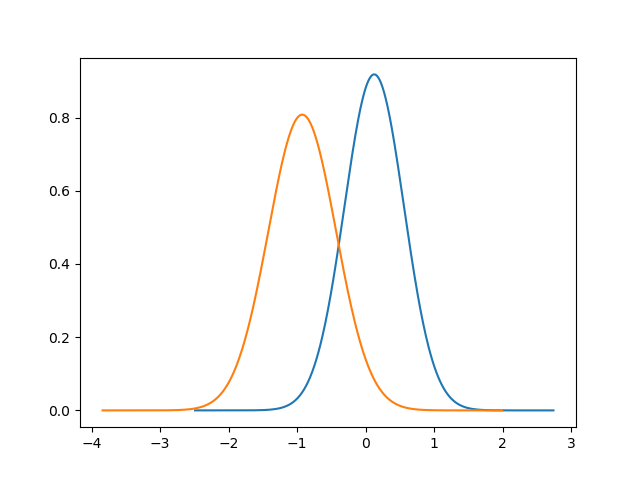
\includegraphics[width=\textwidth]{./Figure_1.png}

\section*{Details zur Implementierung}

In der Fit Methode haben wir beide Kovarianzmatritzen berechnet, als auch die Medians. Anhand der Formel von der
Vorlesung haben wir dann unser Fischer Vektor berechnet. Nachdem, haben wir den Mittelpunkt beider Zentren auf dem
Fischer-Vektor projiziert, damit wir dem später für die Klassifizierung benutzen können.

\begin{lstlisting}[style=py]
    def fit(self, X_train, y_train):
        X_a, X_b = FisherClassifier.split_in_classes(X_train, y_train)
        cov_mat_a = np.cov(X_a, rowvar=False, bias=True)
        cov_mat_b = np.cov(X_b, rowvar=False, bias=True)
        center_a = np.array(X_a, dtype=np.float64).mean(0)
        center_b = np.array(X_b, dtype=np.float64).mean(0)

        alpha = np.linalg.pinv(cov_mat_a + cov_mat_b).dot(center_a - center_b)
        alpha_normalized = alpha / np.linalg.norm(alpha)
        self.alpha = alpha_normalized

        # to determine whether a point belongs to class a or class b we need a threshold
        # on the 1 dimensional space. This one is the projected point between the 2 centers
        self.threshold = self.project_point((center_a + center_b) / 2)

        self.plot_probability_distribution(center_a, center_b, X_a, X_b)

\end{lstlisting}

Die eigentliche Klassifizierung ist ganz simpel. Wir projizieren das neue Punkt auf dem Fischer-Vektor und schauen,
ob es vor oder nach unser in Fit definierten Threshold ist.

\begin{lstlisting}[style=py]
    def predict_single(self, x):
        # project x into alpha (AKA Fisher's vector)
        projected = self.project_point(x)
        return projected < self.threshold
\end{lstlisting}

Die ganze Plot Funktionalität ist nicht so interessant, außer 2 relevante Teile. Wir haben die folgende Funktion
benutzt, um die Dichtefunktion zu berechnen (da bei Fischer Normalverteilung eine Voraussetzung ist)

\begin{lstlisting}[style=py]
@staticmethod
    def get_density_function(center, covariance):
        return lambda x: math.e ** (
            (-1/2) * ((x - center) / covariance) ** 2
        ) / (covariance * math.sqrt((2*math.pi)))
\end{lstlisting}

Dabei brauchen wir aber die Kovarianz. Die wird von alle projizierten Punkten so berechnet.

\begin{lstlisting}[style=py]
@staticmethod
    def get_covariance_for_projected(points, center):
        vectorized_sq_distances_sum = np.vectorize(lambda x, m: (x - m)**2)
        square_distances_sum = np.sum(vectorized_sq_distances_sum(points, center))
        return math.sqrt(square_distances_sum / len(points))
\end{lstlisting}

\section*{Code in FisherClassifier.py}

\begin{lstlisting}[style=py]
from Classifier import Classifier
from Parser import get_data_set
import numpy as np
from sklearn.linear_model import LinearRegression
import math
from random import random
import matplotlib.pyplot as plt
from scipy.stats import multivariate_normal


class FisherClassifier(Classifier):
    def __init__(self, Ximport csv
import numpy as np
import os
from sklearn.model_selection import train_test_split


def parse_data():
    file_name = os.path.join(os.path.dirname(__file__), './Dataset/spambase.data')
    csv_file = open(file_name, 'rt')
    reader = csv.reader(csv_file, delimiter=',', quoting=csv.QUOTE_NONE)
    data = []

    for row in reader:
        filtered = list(filter(lambda x: x != '', row))
        data.append(list(map(lambda x: float(x), filtered)))

    return data


def get_points_and_labels_from_data(data):
    points = np.array(list(map(lambda x: x[:-1], data)), dtype=np.float64)
    labels = np.array(list(map(lambda x: int(x[-1]), data)))

    return points, labels


def get_data_set(seed):
    data = parse_data()
    X, y = get_points_and_labels_from_data(data)
    # for determined results we use a seed for random_state, so that data is always split
    X_train, X_test, y_train, y_test = train_test_split(X, y, train_size=0.8, test_size=0.2,
                                                        random_state=seed)

    return X_train, X_test, y_train, y_test
_train, y_train):
        self.alpha = None
        self.threshold = None
        self.fit(X_train, y_train)

    @staticmethod
    def split_in_classes(X_train, y_train):
        split_X = ([], [])

        for idx, x in enumerate(X_train):
            current_label = y_train[idx]
            split_X[current_label].append(x)

        return split_X

    @staticmethod
    def get_density_function(center, covariance):
        return lambda x: math.e ** (
            (-1/2) * ((x - center) / covariance) ** 2
        ) / (covariance * math.sqrt((2*math.pi)))

    @staticmethod
    def get_covariance_for_projected(points, center):
        vectorized_sq_distances_sum = np.vectorize(lambda x, m: (x - m)**2)
        square_distances_sum = np.sum(vectorized_sq_distances_sum(points, center))
        return math.sqrt(square_distances_sum / len(points))

    def plot_class(self, points, center):
        projected_center = self.project_point(center)
        projected_points = list(map(lambda x: self.project_point(x), points))
        covariance = FisherClassifier.get_covariance_for_projected(projected_points, projected_center)
        density_a = FisherClassifier.get_density_function(projected_center, covariance)
        plot_distance = 5000
        y_of_plot = [density_a(float(x) / 100) for x in range(-plot_distance, plot_distance)]
        x_to_plot = [float(x) / 100 for x in range(-plot_distance, plot_distance)]
        first_decent = None
        last_decent = None

        for idx, y in enumerate(y_of_plot):
            if y > 0.01 and first_decent is None:
                first_decent = idx
            elif y <= 0.01 and first_decent is not None:
                last_decent = idx
                break

        beauty_margin = (last_decent - first_decent)
        start = int(first_decent - beauty_margin/2)
        end = int(last_decent + beauty_margin/2)

        plt.plot(x_to_plot[start:end], y_of_plot[start:end])

    def plot_probability_distribution(self, center_a, center_b, points_a, points_b):
        self.plot_class(points_a, center_a)
        self.plot_class(points_b, center_b)
        plt.show()

    def project_point(self, x):
        return x.dot(self.alpha)

    def fit(self, X_train, y_train):
        X_a, X_b = FisherClassifier.split_in_classes(X_train, y_train)
        cov_mat_a = np.cov(X_a, rowvar=False, bias=True)
        cov_mat_b = np.cov(X_b, rowvar=False, bias=True)
        center_a = np.array(X_a, dtype=np.float64).mean(0)
        center_b = np.array(X_b, dtype=np.float64).mean(0)

        alpha = np.linalg.pinv(cov_mat_a + cov_mat_b).dot(center_a - center_b)
        alpha_normalized = alpha / np.linalg.norm(alpha)
        self.alpha = alpha_normalized

        # to determine whether a point belongs to class a or class b we need a threshold
        # on the 1 dimensional space. This one is the projected point between the 2 centers
        self.threshold = self.project_point((center_a + center_b) / 2)

        self.plot_probability_distribution(center_a, center_b, X_a, X_b)

    def predict(self, X):
        return list(map(lambda x: self.predict_single(x), X))

    def predict_single(self, x):
        # project x into alpha (AKA Fisher's vector)
        projected = self.project_point(x)
        return projected < self.threshold


# max_score = 0
# min_score = 100
# best_seed = 0
# worst_seed = 0

# for i in range(1000):
#     X_train, X_test, y_train, y_test = get_data_set(i)
#     classifier = FisherClassifier(X_train, y_train)
#     score = classifier.score(X_test, y_test)
#     if score > max_score:
#         max_score = score
#         best_seed = i
#     if score < min_score:
#         min_score = score
#         worst_seed = i
#
# print('Best score for seed={}: {}'.format(best_seed, max_score))
# print('Worst score for seed{}: {}'.format(worst_seed, min_score))

X_train, X_test, y_train, y_test = get_data_set(879)
classifier = FisherClassifier(X_train, y_train)
score = classifier.score(X_test, y_test)
print('Score: {}'.format(classifier.score(X_test, y_test)))

lm = LinearRegression()
y_train_modified = list(map(lambda x: 1 if x == 1 else -1, y_train))
lm.fit(X_train, y_train_modified)
prediction = np.array(list(map(lambda x: 1 if x > 0 else 0, lm.predict(X_test))), dtype=np.float64)
score = np.mean(prediction == np.array(y_test, dtype=np.float64))
print('Score with linear regression: {}'.format(score))

\end{lstlisting}

\section*{Code in Parser.py}

\begin{lstlisting}[style=py]
import csv
import numpy as np
import os
from sklearn.model_selection import train_test_split


def parse_data():
    file_name = os.path.join(os.path.dirname(__file__), './Dataset/spambase.data')
    csv_file = open(file_name, 'rt')
    reader = csv.reader(csv_file, delimiter=',', quoting=csv.QUOTE_NONE)
    data = []

    for row in reader:
        filtered = list(filter(lambda x: x != '', row))
        data.append(list(map(lambda x: float(x), filtered)))

    return data


def get_points_and_labels_from_data(data):
    points = np.array(list(map(lambda x: x[:-1], data)), dtype=np.float64)
    labels = np.array(list(map(lambda x: int(x[-1]), data)))

    return points, labels


def get_data_set(seed):
    data = parse_data()
    X, y = get_points_and_labels_from_data(data)
    # for determined results we use a seed for random_state, so that data is always split
    X_train, X_test, y_train, y_test = train_test_split(X, y, train_size=0.8, test_size=0.2,
                                                        random_state=seed)

    return X_train, X_test, y_train, y_test

\end{lstlisting}



% /////////////////////// END DOKUMENT /////////////////////////
\end{document}
